\documentclass[11pt]{article}

\usepackage[margin=0.82in]{geometry}
\usepackage[T1]{fontenc}
\usepackage[utf8]{inputenc}
\usepackage{newtxtext,newtxmath}
\usepackage{microtype}
\usepackage{graphicx}
\usepackage{booktabs}
\usepackage{array}
\usepackage{tabularx}
\usepackage{siunitx}
\usepackage{amsmath,mathtools}
\usepackage{caption}
\usepackage{subcaption}
\usepackage{float}
\usepackage{placeins}
\usepackage{enumitem}
\usepackage{xcolor}
\usepackage{fancyhdr}
\usepackage{titlesec}
\usepackage[hidelinks]{hyperref}
\usepackage{setspace}

\definecolor{navy}{HTML}{18324A}
\definecolor{softgray}{HTML}{F3F5F7}
\definecolor{linegray}{HTML}{C7CDD3}

\hypersetup{
  colorlinks=true,
  linkcolor=navy,
  citecolor=navy,
  urlcolor=navy,
  pdftitle={Computational Design of a Ni-Cr-Al Superalloy Using Thermo-Calc},
  pdfauthor={Jeonghyun Park}
}

\captionsetup{font=small,labelfont=bf,labelsep=period}
\sisetup{detect-all,round-mode=places,round-precision=2}
\setlength{\parindent}{0pt}
\setlength{\parskip}{0.55em}
\setstretch{1.03}
\renewcommand{\arraystretch}{1.15}
\setlist[itemize]{leftmargin=1.4em,itemsep=0.2em,topsep=0.3em}

\titleformat{\section}{\Large\bfseries\color{navy}}{\thesection}{0.6em}{}
\titleformat{\subsection}{\large\bfseries\color{navy}}{\thesubsection}{0.6em}{}
\titleformat{\subsubsection}{\normalsize\bfseries}{\thesubsubsection}{0.5em}{}
\titlespacing*{\section}{0pt}{1.2em}{0.45em}
\titlespacing*{\subsection}{0pt}{0.9em}{0.35em}

\setlength{\headheight}{14pt}
\pagestyle{fancy}
\fancyhf{}
\lhead{MCEN90014 Materials Engineering}
\rhead{Thermo-Calc Design Study}
\cfoot{\thepage}
\renewcommand{\headrulewidth}{0.4pt}

\newcommand{\wtpct}{\ensuremath{\,\mathrm{wt}\%}}
\newcommand{\volfrac}{f_{\mathrm{ppt}}}
\newcommand{\gprime}{\ensuremath{\gamma^{\prime}}}
\newcommand{\gphase}{\ensuremath{\gamma}}
\newcommand{\phase}[1]{\texttt{#1}}

\begin{document}

\begin{titlepage}
\thispagestyle{empty}
\vspace*{1.15in}
{\color{navy}\rule{\textwidth}{1.2pt}}\\[0.35in]
{\Huge\bfseries Computational Design of a Ni--Cr--Al Superalloy Using Thermo-Calc\par}
\vspace{0.22in}
{\Large Phase Stability, Precipitation Strengthening, Oxidation Metric, and Composition Optimization\par}
\vspace{0.38in}
{\color{navy}\rule{\textwidth}{0.7pt}}

\vfill
\begin{tabular}{@{}ll@{}}
\textbf{Author:} & Jeonghyun Park \\
\textbf{Course:} & MCEN90014 Materials Engineering \\
\textbf{Institution:} & The University of Melbourne \\
\textbf{Study type:} & CALPHAD / Thermo-Calc equilibrium design study \\
\textbf{Date:} & May 2026 \\
\end{tabular}
\vfill

\begin{minipage}{0.92\textwidth}
\small
\textbf{Project scope.} Computational screening of heat-treatment response and Ni--Cr--Al composition using equilibrium CALPHAD predictions, assignment-level property models, and constrained composition optimization for a simplified turbine-alloy design problem.
\end{minipage}
\end{titlepage}

\begin{abstract}
Nickel-based superalloys derive high-temperature mechanical capability from a face-centered-cubic \gphase{} matrix strengthened by ordered \gprime{} precipitates while requiring sufficient environmental resistance for service in turbine hardware. This study uses Thermo-Calc equilibrium calculations for the Ni--Cr--Al system to connect heat treatment, phase stability, and composition with two assignment-level property models: precipitation strengthening, $\Delta\sigma = 800\sqrt{\volfrac}$, and an empirical oxidation-resistance metric $k=10^{-4}\exp(-9c_{\mathrm{Al}}-c_{\mathrm{Cr}})$. For the base Ni--16Cr--3.4Al alloy, the prescribed solution treatment at \SI{1050}{\degreeCelsius} lies in the single-phase FCC field, while ageing at \SI{800}{\degreeCelsius} produces an FCC matrix plus \phase{FCC\_L12\#2}, interpreted as \gprime. At \SI{800}{\degreeCelsius}, the base precipitate fraction of 0.08366 corresponds to a calculated strengthening increment of \SI{231.4}{MPa}. Increasing Al raises the \gprime{} fraction but eventually introduces \phase{BCC\_B2}; targeted calculations bracket its sampled onset between 6.89 and 7.00\wtpct{} Al at \SI{800}{\degreeCelsius}. Under the assignment's equal-weight normalization, the best composition in the available Al-only candidate set is Ni--16Cr--4Al, with $\Delta\sigma=\SI{375.7}{MPa}$, $k=5.95\times10^{-5}$, and $PI=1.259$. Allowing both Al and Cr to vary, the strongest tested composition satisfying the 50\wtpct{} precipitate constraint is Ni--15.90Cr--5.44Al, giving 49.98\wtpct{} \phase{FCC\_L12\#2} and $\Delta\sigma=\SI{565.6}{MPa}$. These results define a composition-processing window rather than a stand-alone alloy specification because the calculations are equilibrium-based and do not resolve precipitation kinetics, coarsening, or service-temperature degradation.
\end{abstract}

\section{Introduction}
Nickel-based superalloys are widely used in hot-section turbine components because their microstructures can retain useful strength at temperatures where conventional structural alloys soften rapidly. A central design feature is a continuous Ni-rich FCC \gphase{} matrix containing coherent, ordered L1$_2$ \gprime{} precipitates. The precipitates impede dislocation motion and thereby increase the stress required for plastic deformation. The practical design problem is therefore not simply to maximize the amount of a strengthening phase: the alloy must also remain within a stable and processable phase field and retain adequate resistance to high-temperature oxidation and corrosion \cite{bocchini,grosdidier}.

Heat treatment provides a second design variable. A sufficiently high solution-treatment temperature is used to homogenize the matrix and dissolve secondary phases before cooling to an ageing temperature at which a controlled \gprime{} population becomes thermodynamically favorable. For the simplified Ni--Cr--Al alloy considered here, the prescribed cycle is \SI{1050}{\degreeCelsius} for 2 h followed by \SI{800}{\degreeCelsius} for 16 h. Figure~\ref{fig:heatcycle} summarizes that processing path.

\begin{figure}[H]
    \centering
    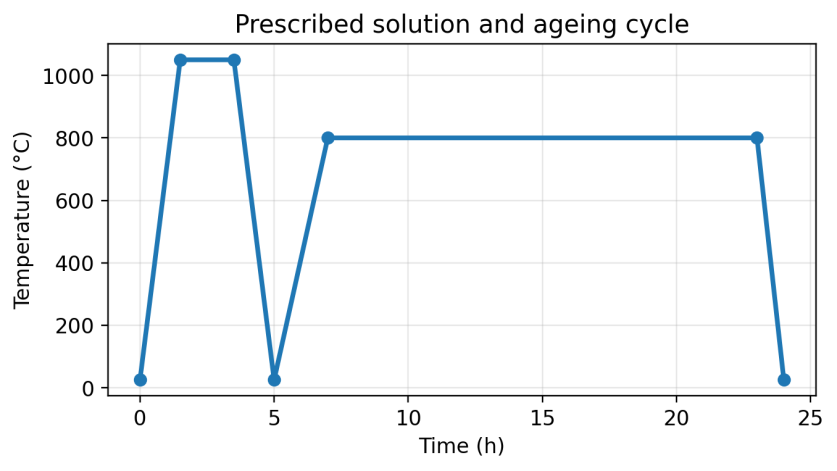
\includegraphics[width=0.73\textwidth]{figures/heat_treatment_cycle.png}
    \caption{Prescribed solution-treatment and ageing cycle used in the assignment.}
    \label{fig:heatcycle}
\end{figure}

CALPHAD calculations are useful for screening this coupled processing-composition space because they predict equilibrium phase assemblages as temperature and chemistry vary. The present study therefore addresses five linked questions: (1) whether the prescribed heat treatment produces the intended \gphase/\gprime{} microstructure; (2) how Al changes phase stability across temperature; (3) how Al alone trades precipitation strengthening against the supplied oxidation metric; (4) how Al and Cr can be co-varied to maximize strengthening while enforcing a 50\wtpct{} precipitate cap; and (5) how the resulting compositions affect a first-order density estimate. The sequence is deliberate: phase stability is established first, then property models are applied only within the resulting design space.

\section{Computational Methodology}
\subsection{Alloy system and calculation plan}
The base composition is Ni--16Cr--3.4Al in mass percent, with Ni treated as the balance. Thermo-Calc equilibrium calculations were used to evaluate the Ni--Cr--Al phase constitution under the calculation sequence in Table~\ref{tab:methodplan}. The reported phase labels are retained from Thermo-Calc; \phase{FCC\_L12} is interpreted as the Ni-rich matrix and \phase{FCC\_L12\#2} as the \gprime-type strengthening precipitate.

\begin{table}[H]
\centering
\caption{Calculation strategy used to connect processing, composition, and the assignment objectives.}
\label{tab:methodplan}
\small
\begin{tabularx}{\textwidth}{@{}p{0.12\textwidth}p{0.22\textwidth}X p{0.24\textwidth}@{}}
\toprule
\textbf{Stage} & \textbf{Variables} & \textbf{Purpose} & \textbf{Primary outputs} \\
\midrule
Q1 & Temperature; base alloy fixed & Verify solution and ageing phase constitution and identify low-temperature competing phases & Equilibrium phase fractions \\
Q2 & Al = 3--8\wtpct; Cr = 16\wtpct; temperature varied & Establish the Al--temperature phase-stability window and identify the emergence of B2 & Phase-boundary map and \SI{800}{\degreeCelsius} section \\
Q3 & Al varied; Cr = 16\wtpct; \SI{800}{\degreeCelsius} & Combine strengthening and empirical oxidation metric under equal weighting & $\Delta\sigma$, $k$, normalized values, performance index \\
Q4 & Al and Cr varied; \SI{800}{\degreeCelsius} & Maximize strengthening while keeping \phase{FCC\_L12\#2} below 50\wtpct{} & Grid search, refined boundary calculations, phase mass fraction \\
Q5 & Candidate compositions & Estimate the effect of composition on mass per unit volume & Ideal additive-volume density \\
\bottomrule
\end{tabularx}
\end{table}

The calculations are equilibrium calculations. Consequently, they identify thermodynamic driving tendencies and stable phase assemblages but do not directly predict precipitation time, nucleation density, precipitate size, coarsening, or whether a low-temperature equilibrium state is reachable within a 16 h ageing treatment. That distinction is important when interpreting the low-temperature results.

\subsection{Property models and optimization metrics}
The supplied strengthening model is
\begin{equation}
\Delta\sigma = S\sqrt{\volfrac}, \qquad S=\SI{800}{MPa},
\label{eq:strength}
\end{equation}
where $\volfrac$ is the precipitate fraction used for the corresponding assignment calculation. The supplied empirical oxidation metric is
\begin{equation}
k = k_0\exp\left(-a c_{\mathrm{Al}}-b c_{\mathrm{Cr}}\right),
\qquad k_0=10^{-4},\quad a=9,\quad b=1,
\label{eq:k}
\end{equation}
with $c_{\mathrm{Al}}$ and $c_{\mathrm{Cr}}$ entered as mass fractions. Following the assignment convention used in the original submission, larger $k$ is treated as the preferred oxidation-resistance metric. For Q3, strength and $k$ are therefore normalized over the sampled candidate set using
\begin{align}
\Delta\sigma_n &= \frac{\Delta\sigma-\Delta\sigma_{\min}}{\Delta\sigma_{\max}-\Delta\sigma_{\min}}, \\
k_n &= \frac{k-k_{\min}}{k_{\max}-k_{\min}}, \\
PI &= \Delta\sigma_n+k_n.
\end{align}
No additional weighting factor is introduced; the two normalized objectives contribute equally.

For Q4, the assignment constraint is expressed in precipitate mass percent. When Thermo-Calc phase masses are available, the constrained fraction is calculated directly as
\begin{equation}
f_{\mathrm{ppt,wt}}=\frac{m(\phase{FCC\_L12\#2})}{m_{\mathrm{total}}}.
\label{eq:massfraction}
\end{equation}
If only phase amount or volume fraction were available, the corresponding mass fraction would require conversion using phase molar mass or phase density, respectively.

\section{Results and Discussion}
\subsection{Q1: Effect of temperature on the base alloy}
The base-alloy temperature sweeps are most informative when the high-temperature dissolution behavior and the lower-temperature competing phases are viewed together. Figure~\ref{fig:tempsweeps} therefore combines the two original temperature calculations rather than presenting them as disconnected figures.

\begin{figure}[H]
\centering
\begin{subfigure}[t]{0.49\textwidth}
    \centering
    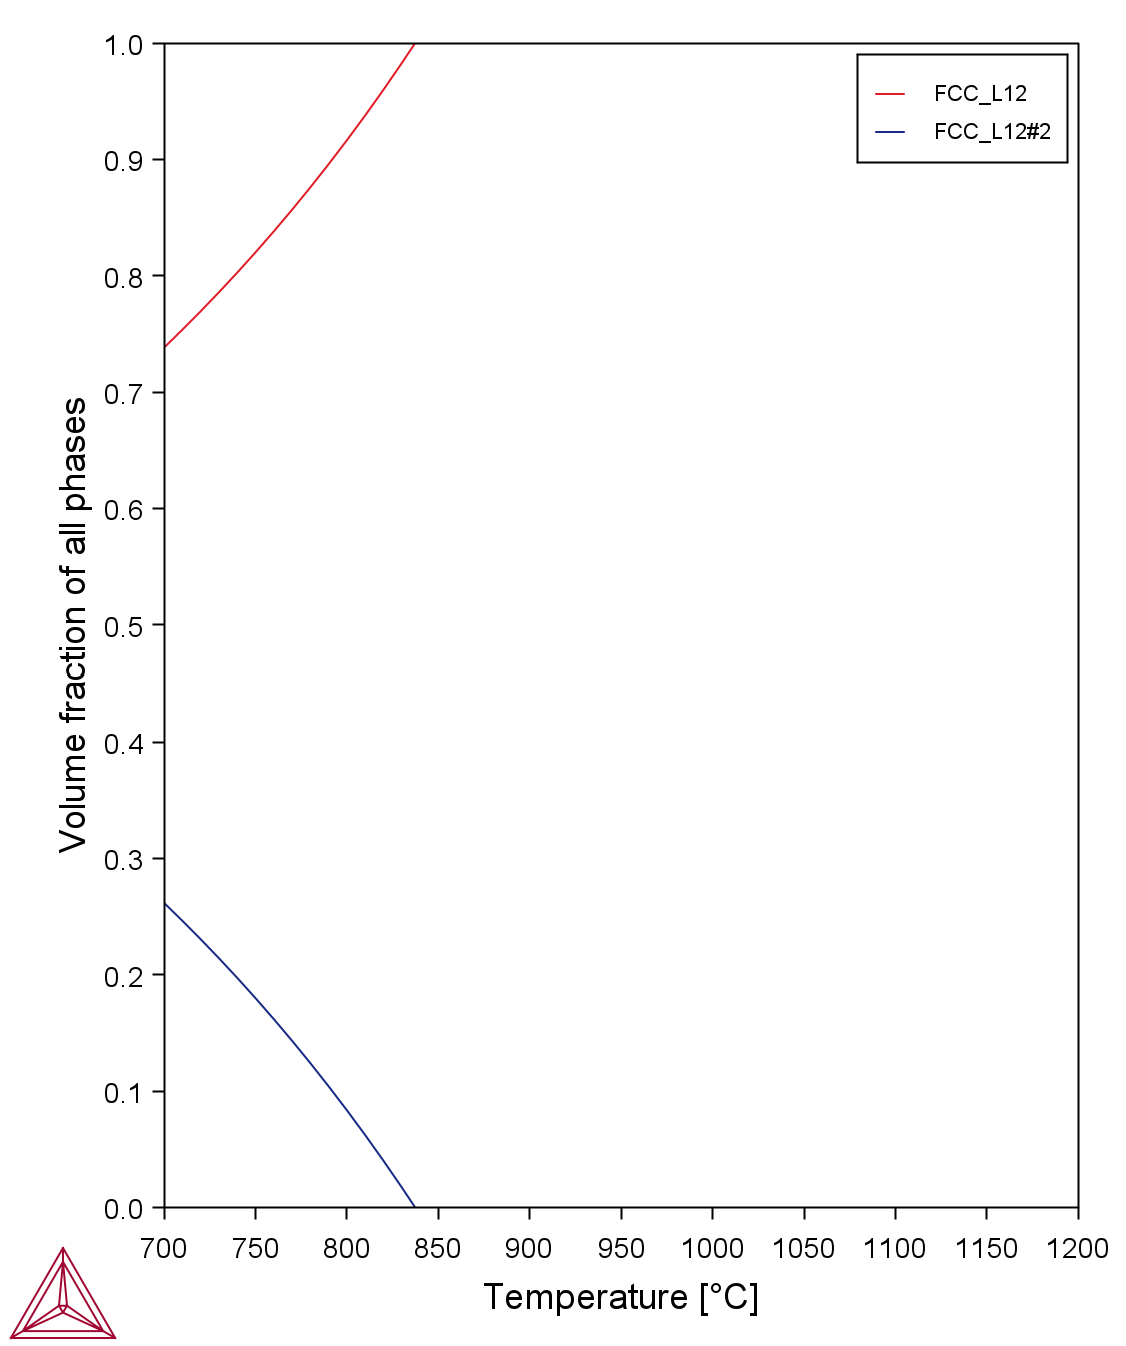
\includegraphics[width=\linewidth]{figures/temp_sweep_high.png}
    \caption{High-temperature sweep resolving the disappearance of \phase{FCC\_L12\#2}.}
\end{subfigure}\hfill
\begin{subfigure}[t]{0.49\textwidth}
    \centering
    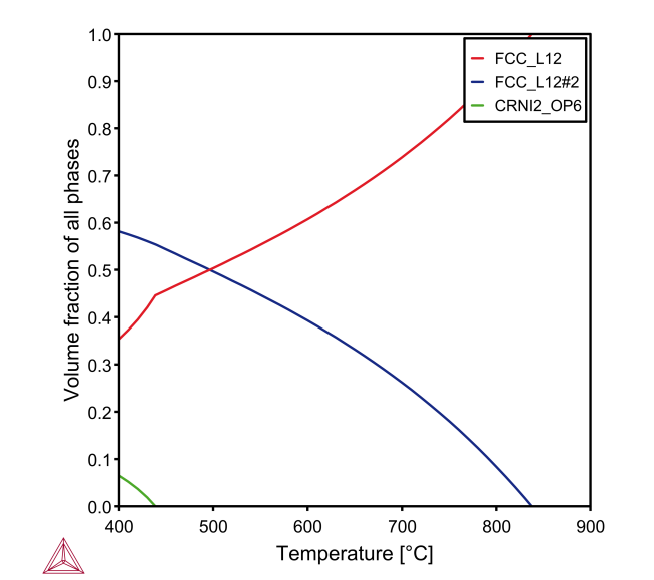
\includegraphics[width=\linewidth]{figures/temp_sweep_low.png}
    \caption{Lower-temperature sweep showing both the increasing \phase{FCC\_L12\#2} fraction and the additional \phase{CRNI2\_OP6} phase.}
\end{subfigure}
\caption{Equilibrium phase fractions of Ni--16Cr--3.4Al as a function of temperature. The two panels serve complementary purposes: panel (a) resolves the \gprime{} solvus and solution-treatment condition, whereas panel (b) exposes phases that would be missed by a high-temperature-only sweep.}
\label{fig:tempsweeps}
\end{figure}

At \SI{1050}{\degreeCelsius}, the calculated equilibrium state is single-phase \phase{FCC\_L12}. This supports the prescribed solution treatment because a single FCC field is consistent with dissolving the strengthening precipitate before ageing. At \SI{800}{\degreeCelsius}, the calculation predicts coexistence of \phase{FCC\_L12} and \phase{FCC\_L12\#2}, which is interpreted as the target \gphase+\gprime{} microstructure. The calculated precipitate fraction at the ageing condition is 0.08366, giving
\begin{equation}
\Delta\sigma_{800} = 800\sqrt{0.08366}=\SI{231.4}{MPa}.
\end{equation}
The high-temperature sweep further shows that \phase{FCC\_L12\#2} vanishes above the mid-\SI{800}{\degreeCelsius} range, so ageing too close to or above that solvus would reduce the equilibrium precipitate fraction and therefore reduce the strengthening contribution predicted by Eq.~\ref{eq:strength}.

The lower-temperature calculation adds an important qualification. \phase{CRNI2\_OP6} appears at the low-temperature end of the sweep and disappears well before the prescribed \SI{800}{\degreeCelsius} ageing condition. Its presence means that lowering the ageing temperature cannot be interpreted as a monotonic route to ``more \gprime{} and therefore more strength.'' At sufficiently low temperature the equilibrium phase assemblage itself changes. In addition, the thermodynamic prediction does not establish whether such low-temperature equilibrium can form within 16 h because diffusion and precipitation kinetics are not modeled. The prescribed \SI{800}{\degreeCelsius} ageing temperature is therefore best interpreted as a compromise within a clean \gphase+\gprime{} field rather than as an equilibrium-strength maximum.

\subsection{Q2: Effect of aluminium across temperature and phase stability}
Al affects both the amount of strengthening precipitate and the boundaries of the phase fields. Figure~\ref{fig:almap} first shows the full Al--temperature map at fixed 16\wtpct{} Cr; the \SI{800}{\degreeCelsius} phase-fraction section is then used to quantify the trend relevant to the prescribed ageing treatment.

\begin{figure}[H]
\centering
\begin{subfigure}[t]{0.48\textwidth}
    \centering
    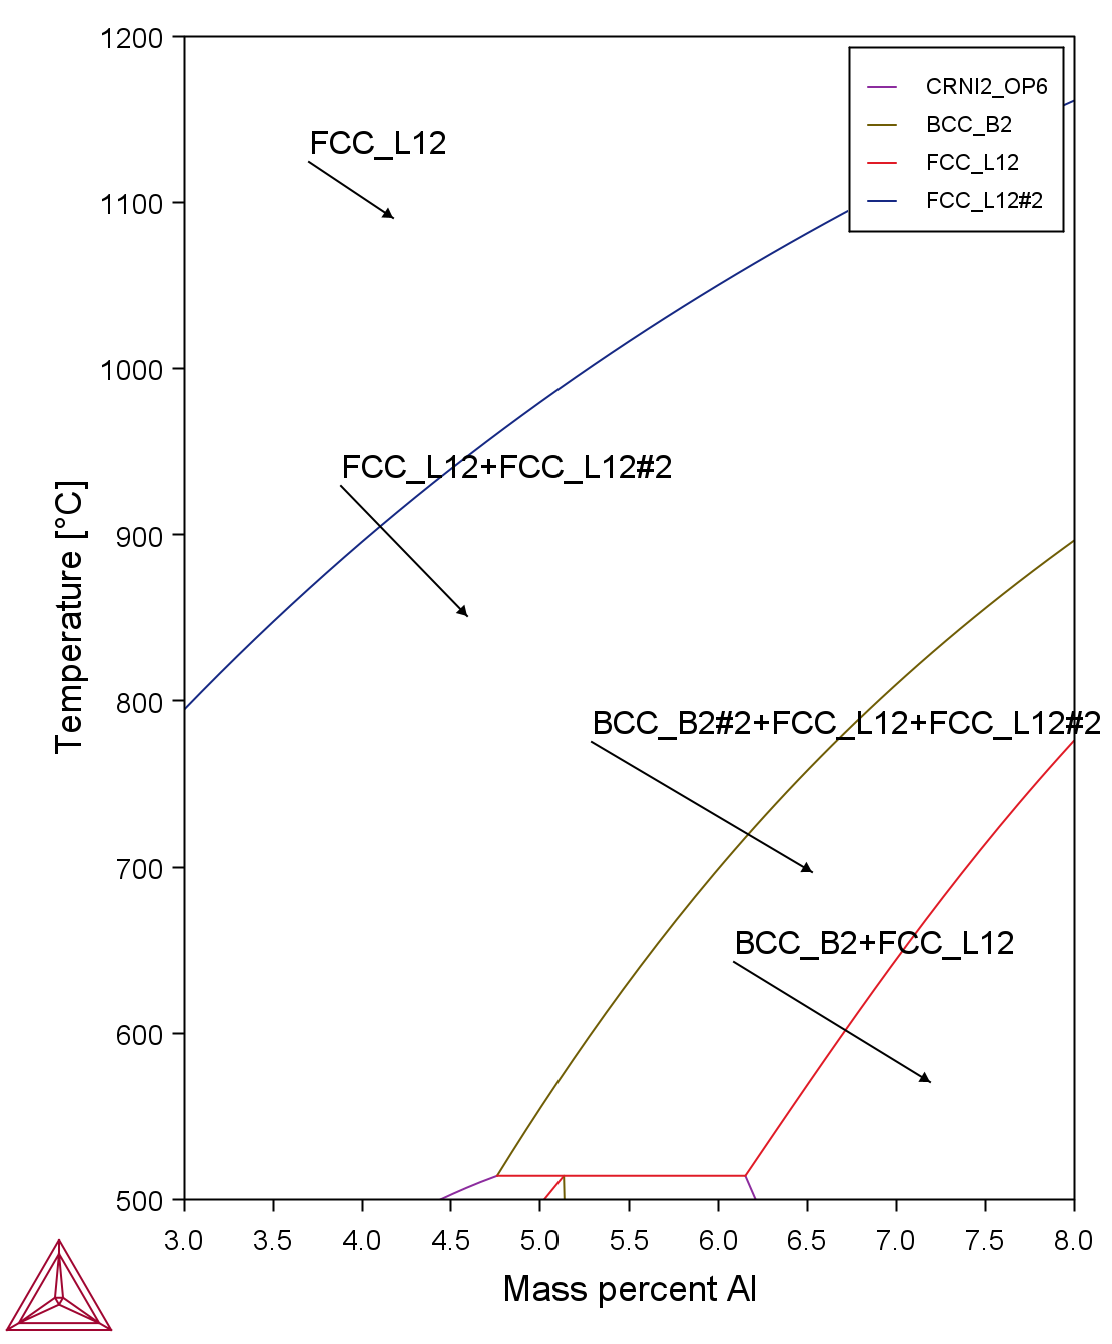
\includegraphics[width=\linewidth]{figures/al_temperature_map.png}
    \caption{Al--temperature phase-boundary map at 16\wtpct{} Cr.}
\end{subfigure}\hfill
\begin{subfigure}[t]{0.50\textwidth}
    \centering
    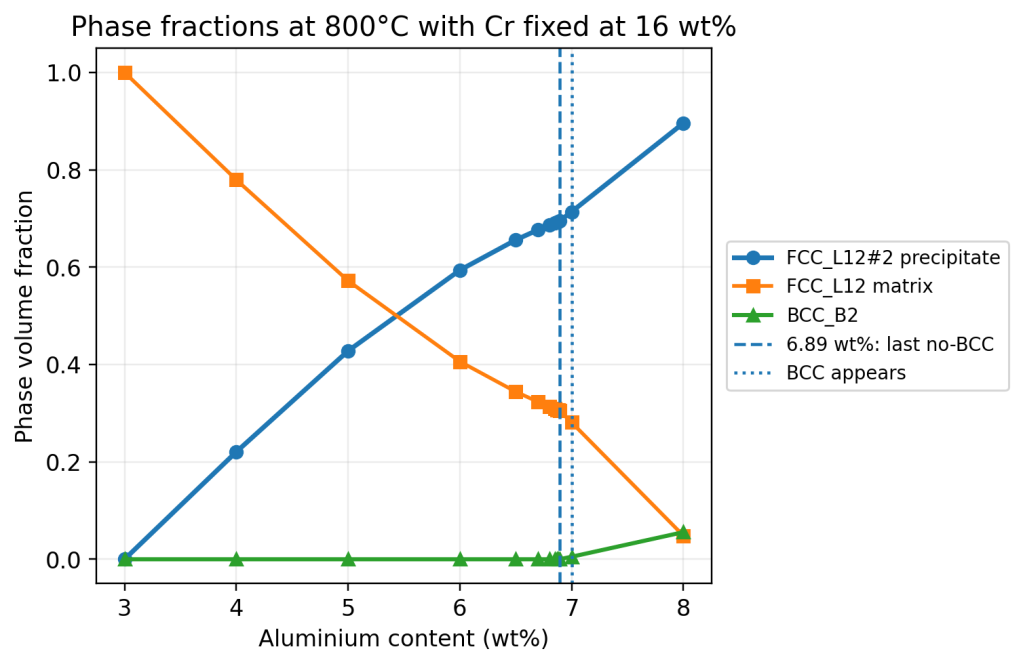
\includegraphics[width=\linewidth]{figures/al_sweep_800.png}
    \caption{Phase fractions along the \SI{800}{\degreeCelsius} section.}
\end{subfigure}
\caption{Effect of Al on phase stability. The phase map supplies the multi-temperature context, while the \SI{800}{\degreeCelsius} section quantifies the composition trend at the prescribed ageing condition.}
\label{fig:almap}
\end{figure}

Across the map, increasing Al raises the temperature range over which \phase{FCC\_L12\#2} is stable, consistent with Al promoting the ordered strengthening phase. At \SI{800}{\degreeCelsius}, the calculated \phase{FCC\_L12\#2} fraction rises strongly as Al increases from 3 to 8\wtpct{}, while the matrix fraction correspondingly decreases. This is beneficial to the precipitation-strengthening model but cannot be extended indefinitely because a B2-containing phase field enters at higher Al.

The targeted high-Al calculations refine that transition. Figure~\ref{fig:b2onset} shows that 6.89\wtpct{} Al is the last sampled composition without B2, while the tabulated 7.00\wtpct{} calculation contains a \phase{BCC\_B2} volume fraction of 0.0052. Thus the sampled onset of \phase{BCC\_B2} at \SI{800}{\degreeCelsius} is bracketed between 6.89 and 7.00\wtpct{} Al rather than described only as ``approximately 7\wtpct.''

\begin{figure}[H]
    \centering
    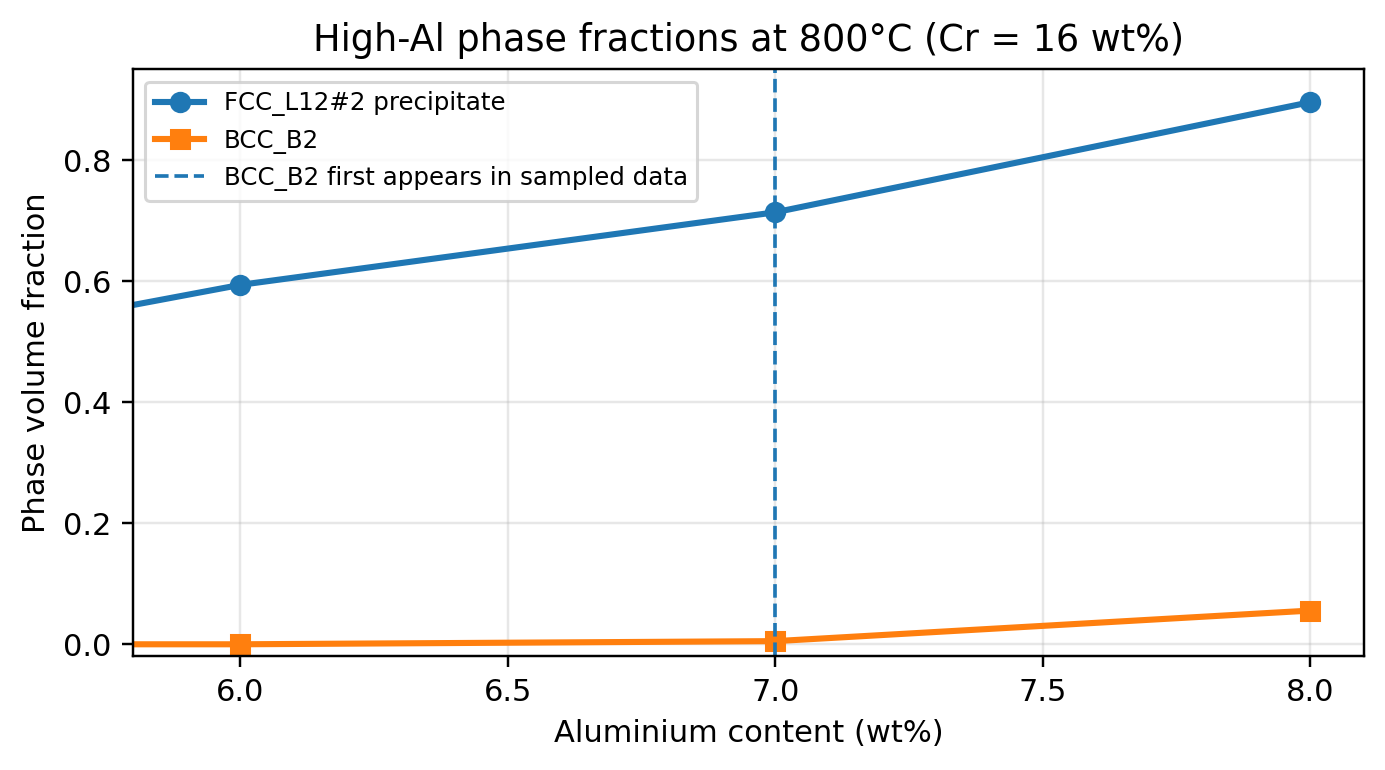
\includegraphics[width=0.80\textwidth]{figures/high_al_b2.png}
    \caption{Targeted high-Al calculations at \SI{800}{\degreeCelsius} and 16\wtpct{} Cr. The additional sampling is used to bracket the first appearance of \phase{BCC\_B2}.}
    \label{fig:b2onset}
\end{figure}

The B2-containing region is excluded from the preferred design space because the target microstructure is an FCC matrix strengthened by controlled L1$_2$ precipitates. A second ordered intermetallic phase changes both the deformation mechanisms and the processing window; NiAl-type B2 phases are also associated with limited low-temperature tensile ductility in monolithic form \cite{noebe}. Q2 therefore provides the phase-stability constraint needed before the Q3 property trade-off is evaluated.

\subsection{Q3: Al-only multi-objective screening at \SI{800}{\degreeCelsius}}
For Q3, Cr remains fixed at 16\wtpct{} and the heat treatment remains fixed at \SI{1050}{\degreeCelsius} solution treatment followed by \SI{800}{\degreeCelsius} ageing. The available candidate calculations are summarized in Table~\ref{tab:q3}. Presenting the complete property table here avoids separating the Q3 data from the Q3 interpretation.

\begin{table}[H]
\centering
\caption{Q3 sampled candidates at \SI{800}{\degreeCelsius}. Normalization is performed only over this six-point candidate set.}
\label{tab:q3}
\small
\begin{tabular}{@{}rrrrrrrr@{}}
\toprule
Al (wt\%) & \phase{FCC\_L12\#2} VF & \phase{BCC\_B2} VF & $\Delta\sigma$ (MPa) & $k$ & $\Delta\sigma_n$ & $k_n$ & PI \\
\midrule
3.00 & 0.0000 & 0.0000 & 0.0   & $6.51\times10^{-5}$ & 0.000 & 1.000 & 1.000 \\
4.00 & 0.2206 & 0.0000 & 375.7 & $5.95\times10^{-5}$ & 0.496 & 0.763 & 1.259 \\
5.00 & 0.4279 & 0.0000 & 523.3 & $5.43\times10^{-5}$ & 0.691 & 0.542 & 1.233 \\
6.00 & 0.5938 & 0.0000 & 616.5 & $4.97\times10^{-5}$ & 0.814 & 0.347 & 1.161 \\
7.00 & 0.7138 & 0.0052 & 675.9 & $4.54\times10^{-5}$ & 0.893 & 0.165 & 1.058 \\
8.00 & 0.8958 & 0.0557 & 757.2 & $4.15\times10^{-5}$ & 1.000 & 0.000 & 1.000 \\
\bottomrule
\end{tabular}
\end{table}

For example, at 4\wtpct{} Al,
\begin{align}
\Delta\sigma &= 800\sqrt{0.2206}=\SI{375.7}{MPa},\\
k &= 10^{-4}\exp[-9(0.040)-0.160]=5.95\times10^{-5},\\
\Delta\sigma_n &= 0.496,\qquad k_n=0.763,\qquad PI=1.259.
\end{align}
Figure~\ref{fig:pi} makes the trade-off explicit: the normalized strength term increases with Al, while the normalized empirical $k$ term decreases. The largest PI among the available sampled candidates occurs at 4\wtpct{} Al, corresponding to Ni--16Cr--4Al.

\begin{figure}[H]
    \centering
    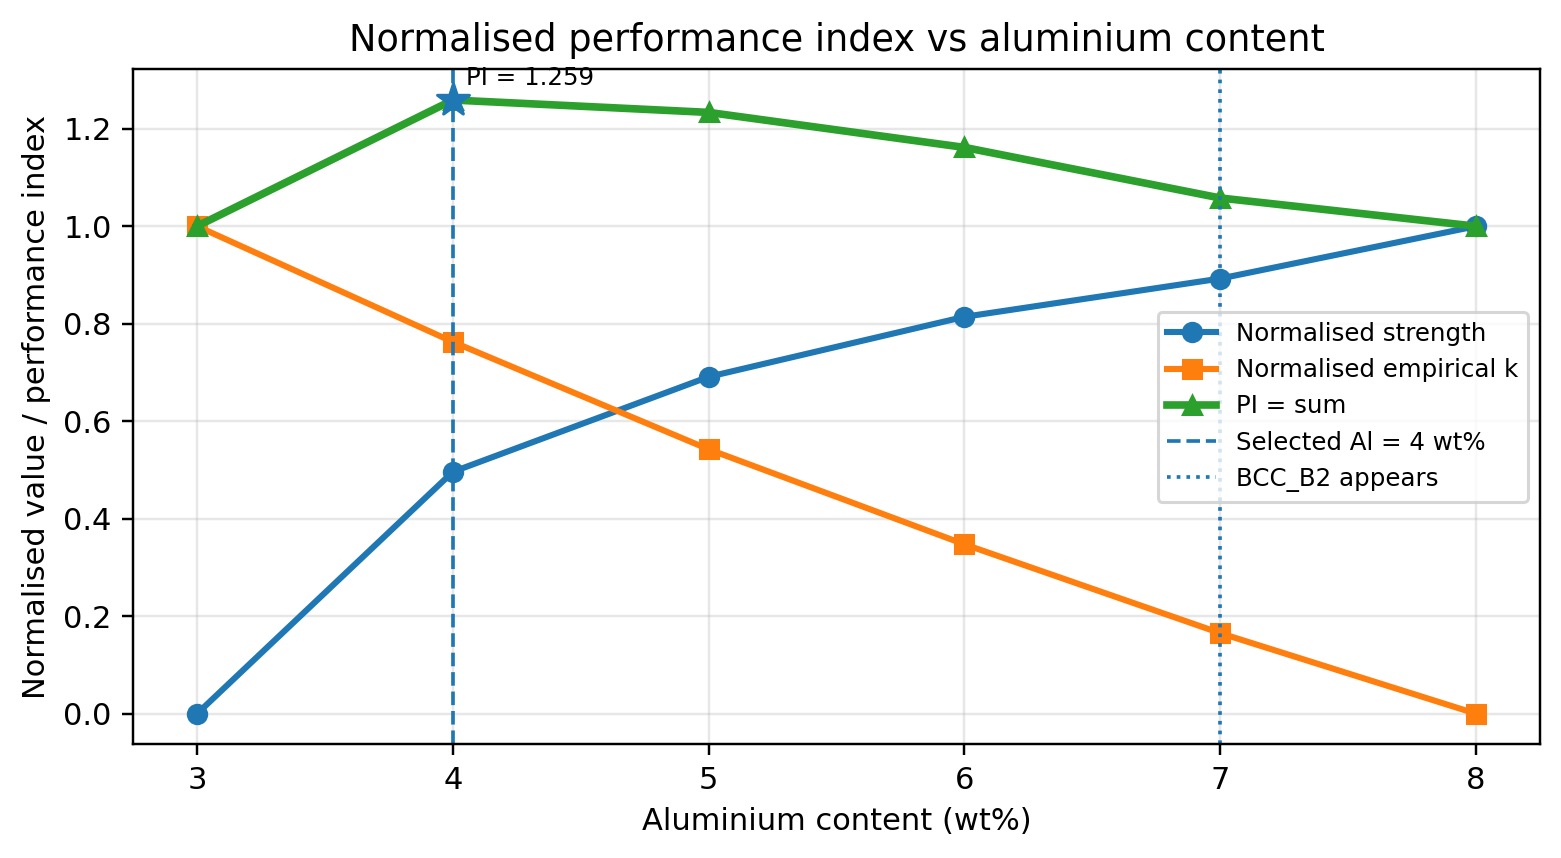
\includegraphics[width=0.79\textwidth]{figures/performance_index.png}
    \caption{Normalized strengthening, normalized empirical oxidation metric, and their equal-weight sum for the available Q3 candidate calculations.}
    \label{fig:pi}
\end{figure}

This result must be described precisely as a \emph{sampled optimum}. The six Q3 points are sufficient to compare the listed candidates, but they are not dense enough to establish that 4.00\wtpct{} Al is the exact maximum of a continuous composition function. A higher-resolution Thermo-Calc sweep around the 4--5\wtpct{} region would be required before claiming a continuous optimum. The present report therefore uses ``best sampled composition'' rather than overstating the resolution of the available data.

\subsection{Q4: Al--Cr strength maximization at \SI{800}{\degreeCelsius}}
Q4 adds Cr as a second composition variable and maximizes the strengthening contribution subject to the assignment constraint that the \phase{FCC\_L12\#2} precipitate remain below 50\wtpct{}. Because Eq.~\ref{eq:strength} increases monotonically with precipitate fraction, the strongest feasible candidate lies as close as possible to the 50\wtpct{} boundary from below.

The initial Al--Cr grid was used to identify the high-precipitate region, after which the search was restricted to the 5--6\wtpct{} Al and 15--17\wtpct{} Cr subdomain. Figures~\ref{fig:q4grids}a--b show this two-stage search. Final single-equilibrium calculations then resolved the mass-fraction boundary near 5.4\wtpct{} Al, as shown in Figure~\ref{fig:q4boundary}.

\begin{figure}[H]
\centering
\begin{subfigure}[t]{0.49\textwidth}
    \centering
    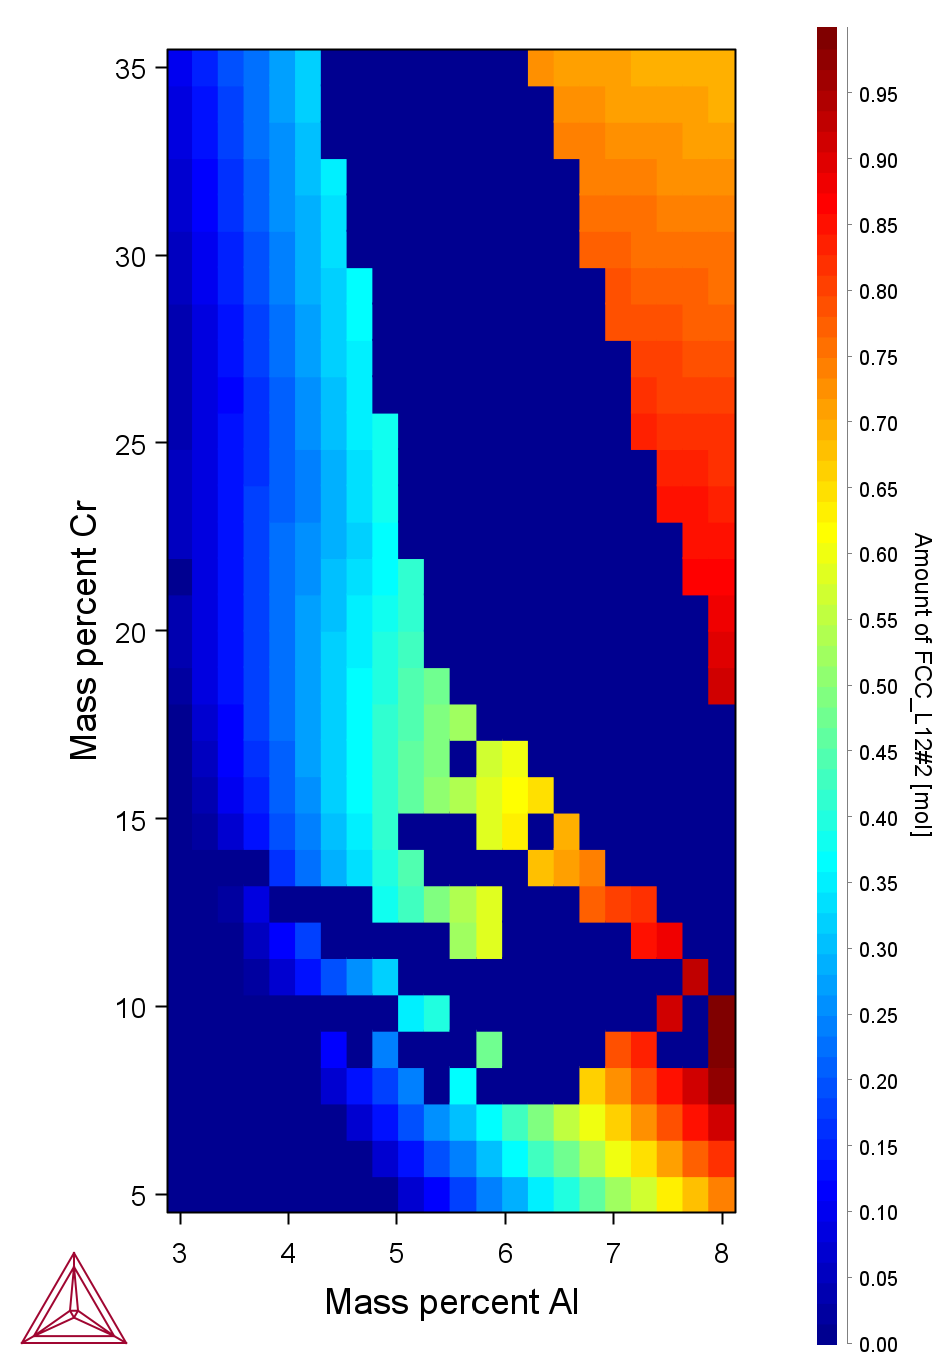
\includegraphics[width=\linewidth]{figures/q4_grid_full.png}
    \caption{Initial Al--Cr grid.}
\end{subfigure}\hfill
\begin{subfigure}[t]{0.49\textwidth}
    \centering
    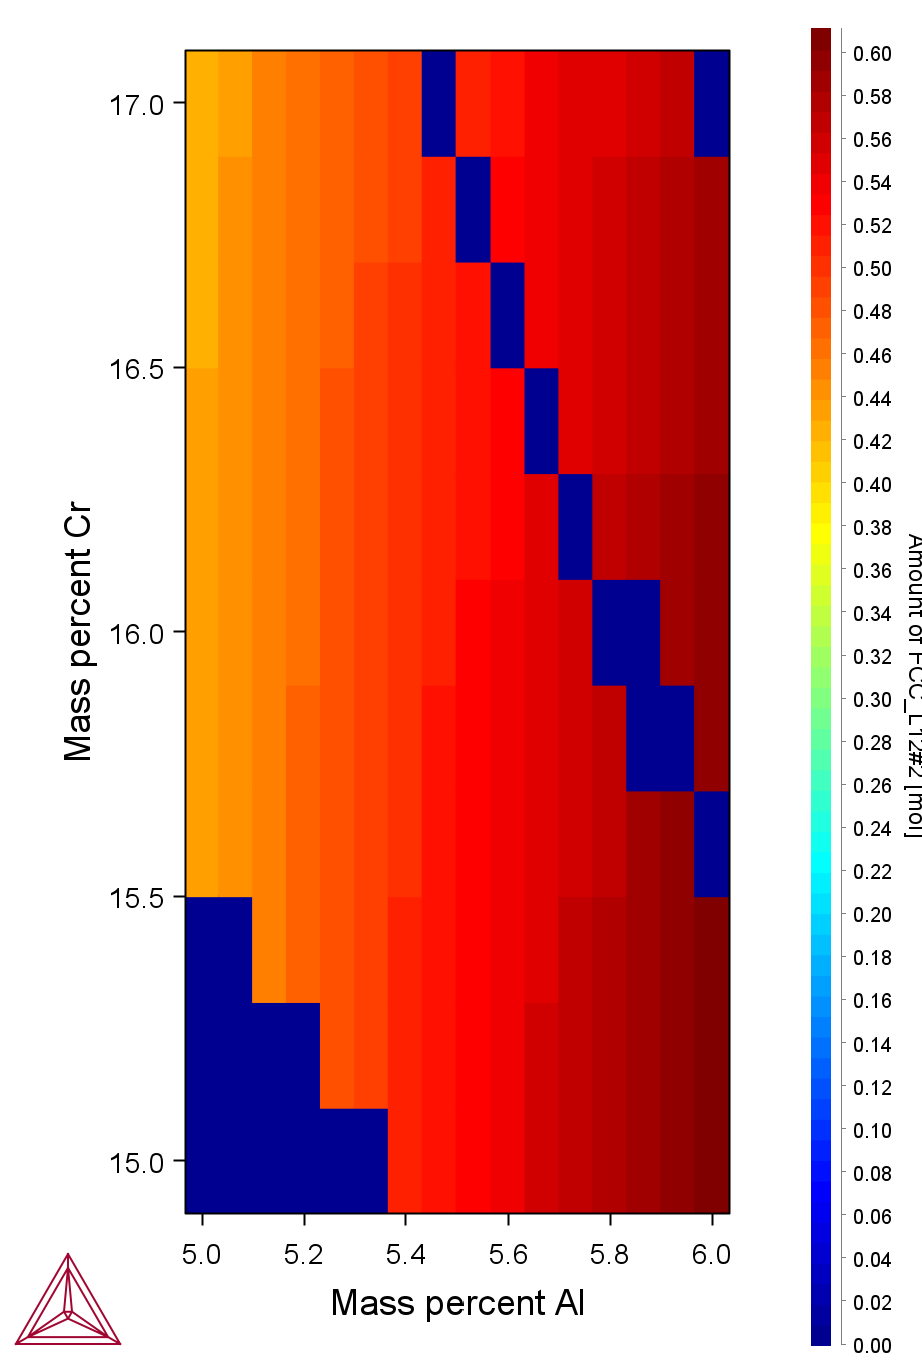
\includegraphics[width=\linewidth]{figures/q4_grid_zoom.png}
    \caption{Refined 5--6\wtpct{} Al, 15--17\wtpct{} Cr region.}
\end{subfigure}
\caption{Two-stage Q4 grid search at \SI{800}{\degreeCelsius}. The grid calculations locate the relevant neighborhood before the final mass-fraction boundary search.}
\label{fig:q4grids}
\end{figure}

\begin{figure}[H]
    \centering
    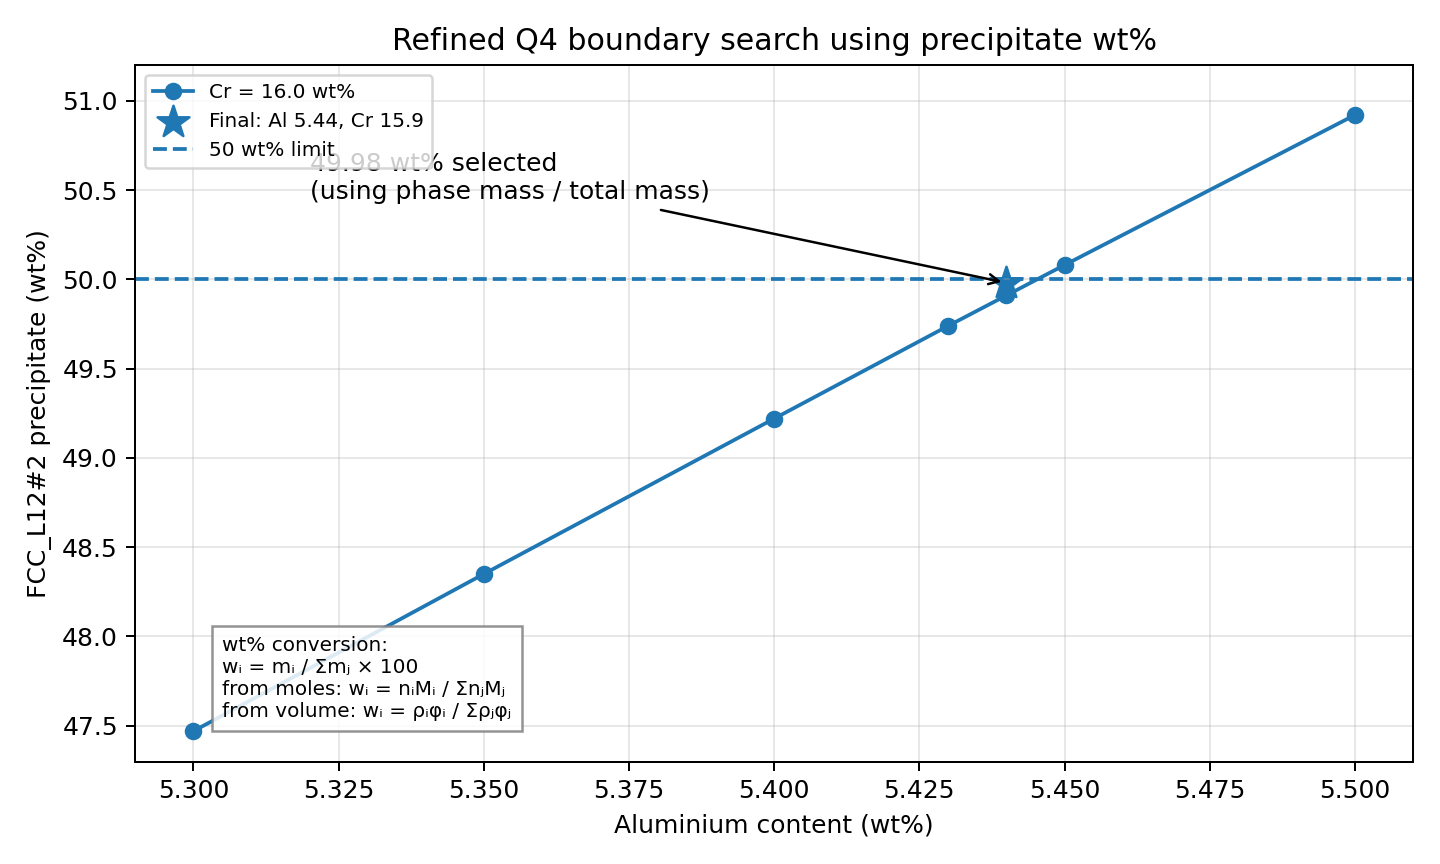
\includegraphics[width=0.83\textwidth]{figures/q4_boundary.png}
    \caption{Final Q4 boundary search using \phase{FCC\_L12\#2} precipitate mass percent.}
    \label{fig:q4boundary}
\end{figure}

The final boundary calculations are reported in Table~\ref{tab:q4}. At fixed Cr = 16.00\wtpct{}, increasing Al from 5.44 to 5.45\wtpct{} moves the precipitate fraction from 49.91 to 50.08\wtpct{}, crossing the constraint. A second calculation at Al = 5.44\wtpct{} and Cr = 15.90\wtpct{} gives 49.98\wtpct{} precipitate, which is the closest tested value below the limit.

\begin{table}[H]
\centering
\caption{Q4 boundary calculations at \SI{800}{\degreeCelsius} using precipitate mass fraction.}
\label{tab:q4}
\small
\begin{tabular}{@{}rrrrrrr@{}}
\toprule
Al & Cr & Ni balance & Total mass & \phase{FCC\_L12\#2} mass & \phase{FCC\_L12\#2} & $\Delta\sigma$ \\
(wt\%) & (wt\%) & (wt\%) & (g) & (g) & (wt\%) & (MPa) \\
\midrule
5.30 & 16.00 & 78.70 & 54.19798 & 25.73033 & 47.47 & 551.2 \\
5.35 & 16.00 & 78.65 & 54.16859 & 26.19301 & 48.35 & 556.3 \\
5.40 & 16.00 & 78.60 & 54.13923 & 26.64888 & 49.22 & 561.3 \\
5.43 & 16.00 & 78.57 & 54.12163 & 26.91908 & 49.74 & 564.2 \\
5.44 & 16.00 & 78.56 & 54.11576 & 27.00858 & 49.91 & 565.2 \\
5.45 & 16.00 & 78.55 & 54.10990 & 27.09780 & 50.08 & 566.1 \\
5.50 & 16.00 & 78.50 & 54.08060 & 27.53964 & 50.92 & 570.9 \\
\textbf{5.44} & \textbf{15.90} & \textbf{78.66} & \textbf{54.12219} & \textbf{27.05012} & \textbf{49.98} & \textbf{565.6} \\
\bottomrule
\end{tabular}
\end{table}

For the selected tested composition,
\begin{align}
f_{\mathrm{ppt,wt}} &= \frac{27.05012}{54.12219}=0.4998,\\
\Delta\sigma &= 800\sqrt{0.4998}=\SI{565.6}{MPa}.
\end{align}
The resulting composition is Ni--15.90Cr--5.44Al (wt\%). A targeted check in the relevant Q4 region showed no \phase{BCC\_B2} formation for the selected candidate, so it satisfies both the explicit 50\wtpct{} precipitate limit and the desired FCC-based phase-stability criterion within the tested conditions.

\subsection{Q5: Effect of alloying on density}
The original draft used a direct mass-fraction-weighted average of elemental densities. Because the listed alloy compositions are mass fractions, a more consistent first-order estimate assumes additive constituent volumes and uses
\begin{equation}
\frac{1}{\rho_{\mathrm{mix}}}=\sum_i \frac{w_i}{\rho_i}.
\label{eq:density}
\end{equation}
Using $\rho_{\mathrm{Ni}}=\SI{8.91}{g.cm^{-3}}$, $\rho_{\mathrm{Cr}}=\SI{7.19}{g.cm^{-3}}$, and $\rho_{\mathrm{Al}}=\SI{2.70}{g.cm^{-3}}$, Eq.~\ref{eq:density} gives the estimates in Table~\ref{tab:density} and Figure~\ref{fig:density}.

\begin{table}[H]
\centering
\caption{First-order density estimates assuming ideal additive volumes.}
\label{tab:density}
\begin{tabular}{@{}lcc@{}}
\toprule
\textbf{Composition} & \textbf{Estimated density (g/cm$^3$)} & \textbf{Change from base} \\
\midrule
Ni--16Cr--3.4Al (base) & 7.98 & --- \\
Ni--16Cr--4Al (Q3) & 7.88 & $-1.22\%$ \\
Ni--15.90Cr--5.44Al (Q4) & 7.66 & $-4.01\%$ \\
\bottomrule
\end{tabular}
\end{table}

\begin{figure}[H]
    \centering
    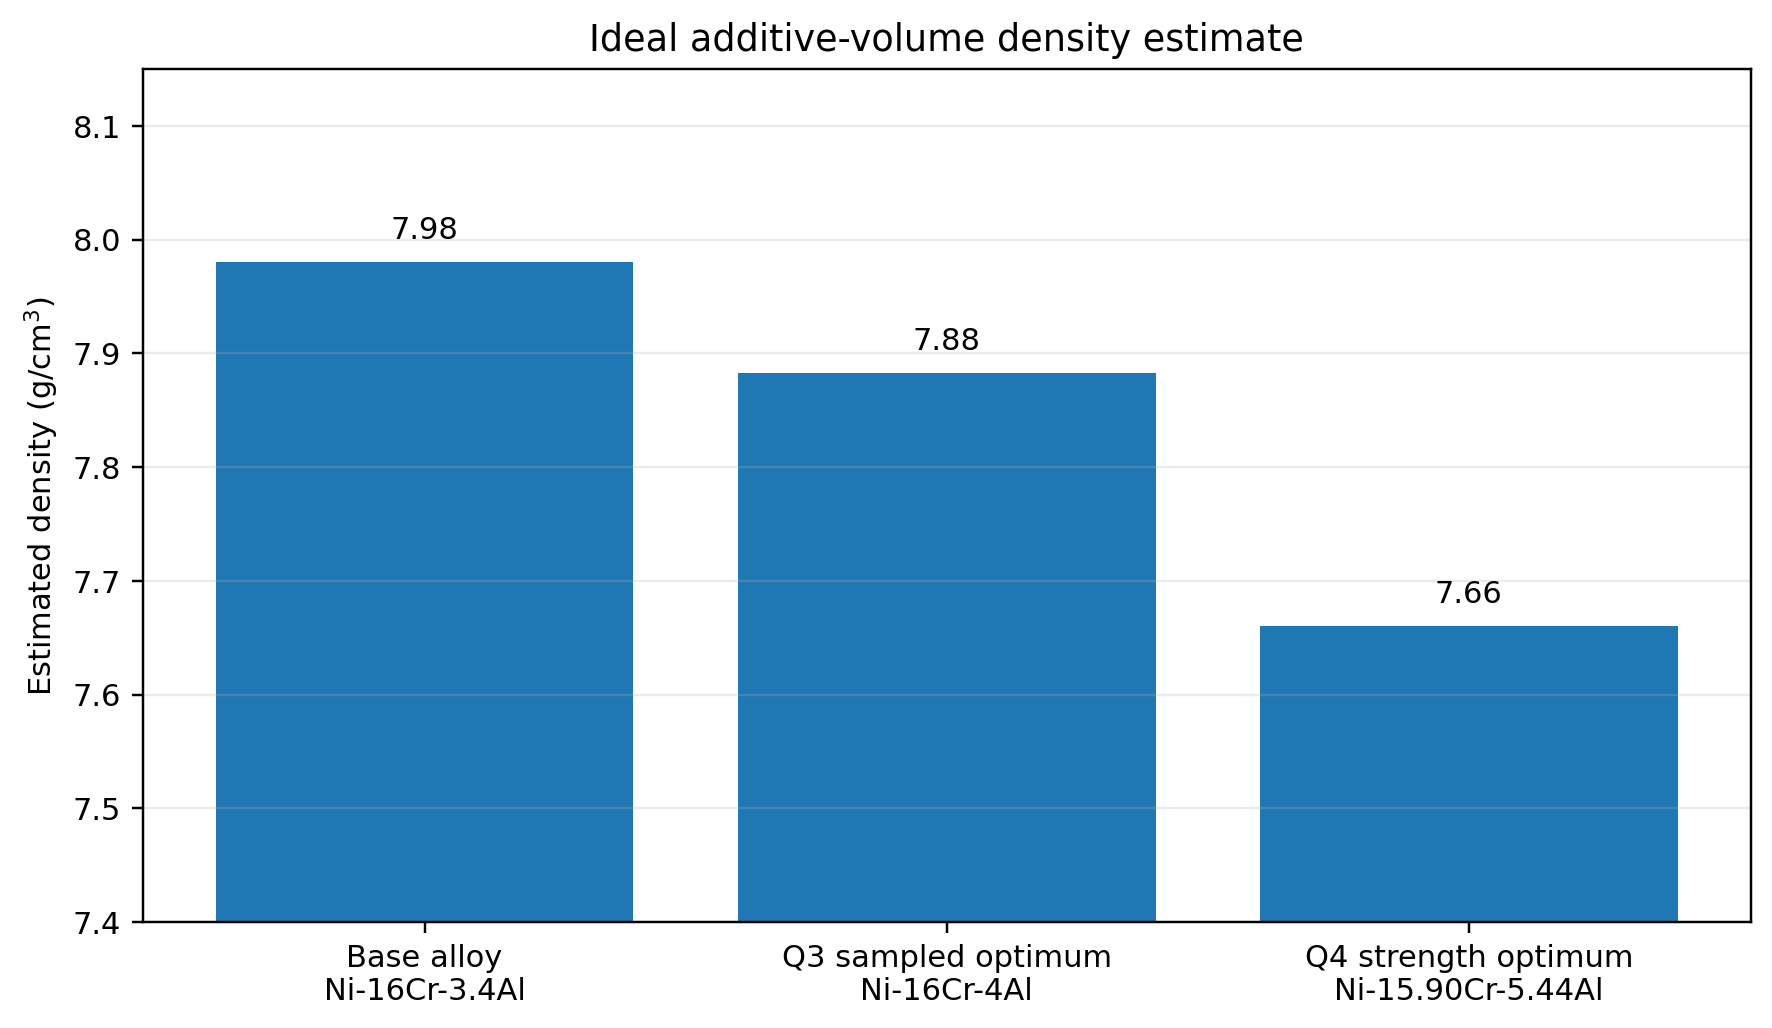
\includegraphics[width=0.74\textwidth]{figures/density_corrected.png}
    \caption{Estimated density of the base alloy and the two selected design compositions using the additive-specific-volume approximation.}
    \label{fig:density}
\end{figure}

Both selected compositions are predicted to reduce density because additional Al replaces denser Ni. For rotating turbine hardware, lower density can reduce centrifugal loading at a given geometry and rotational speed. The estimate should nevertheless be treated as comparative rather than as a substitute for a CALPHAD molar-volume model or measured alloy density.

\section{Engineering Interpretation and Limitations}
The calculations define a useful processing-composition window, but they should not be interpreted as a complete turbine-blade qualification. Four limitations are particularly important:
\begin{itemize}
    \item \textbf{Equilibrium versus kinetics.} Thermo-Calc equilibrium phase fractions do not predict whether the equilibrium amount of \gprime{} forms during a finite 16 h ageing treatment, nor do they predict precipitate size or coarsening.
    \item \textbf{Strength model resolution.} Equation~\ref{eq:strength} reduces precipitation strengthening to a single phase-fraction term. Real strength also depends on precipitate size, coherency, antiphase-boundary energy, dislocation mechanism, grain structure, and temperature.
    \item \textbf{Discrete Q3 sampling.} The reported 4\wtpct{} Al result is the best of the available candidates, not a proven continuous optimum. Additional Thermo-Calc points around the local maximum are needed for a composition-resolution claim finer than 1\wtpct{} Al.
    \item \textbf{Environmental metric.} The $k$ model is an assignment-level empirical metric and is used here exactly under the stated normalization convention. It is not a substitute for oxidation kinetics, scale adhesion, or cyclic environmental testing.
\end{itemize}

These limitations do not invalidate the design exercise; instead, they clarify what each computational result can and cannot support. The strongest conclusion is therefore a screened design recommendation for subsequent higher-fidelity thermodynamic, kinetic, and experimental evaluation.

\section{Conclusions}
Table~\ref{tab:keyresults} collects the key numerical results that define the final design interpretation.

\begin{table}[H]
\centering
\caption{Key results of the Thermo-Calc design study.}
\label{tab:keyresults}
\small
\begin{tabularx}{\textwidth}{@{}p{0.27\textwidth}p{0.24\textwidth}X@{}}
\toprule
\textbf{Question} & \textbf{Key result} & \textbf{Engineering interpretation} \\
\midrule
Base alloy at \SI{1050}{\degreeCelsius} & Single \phase{FCC\_L12} & Supports solution treatment in a homogeneous FCC field. \\
Base alloy at \SI{800}{\degreeCelsius} & $\volfrac=0.08366$, $\Delta\sigma=\SI{231.4}{MPa}$ & Prescribed ageing produces the intended FCC matrix + \gprime-type precipitate. \\
Al phase stability & No B2 at 6.89\wtpct{} Al; B2 present at 7.00\wtpct{} Al & Sampled B2 onset at \SI{800}{\degreeCelsius} is bracketed between these compositions. \\
Q3 sampled optimum & Ni--16Cr--4Al; $\Delta\sigma=\SI{375.7}{MPa}$; $k=5.95\times10^{-5}$; $PI=1.259$ & Best equal-weight candidate among the available Al-only calculations; finer sampling is needed for a continuous optimum. \\
Q4 strength optimum & Ni--15.90Cr--5.44Al; 49.98\wtpct{} precipitate; $\Delta\sigma=\SI{565.6}{MPa}$ & Closest tested candidate below the 50\wtpct{} precipitate constraint, with no B2 detected in the relevant tested region. \\
Density implication & 7.66 g/cm$^3$ for Q4 estimate & About 4.0\% below the base-alloy ideal-mixture estimate. \\
\bottomrule
\end{tabularx}
\end{table}

Overall, the prescribed heat treatment is thermodynamically consistent with a solution-treated FCC matrix followed by \gprime{} precipitation during ageing. Al is an effective lever for increasing the equilibrium precipitate fraction, but its useful range is bounded by the emergence of B2 and by the competing empirical oxidation objective. Under the available Q3 data, Ni--16Cr--4Al gives the largest equal-weight performance index, while the two-variable Q4 search identifies Ni--15.90Cr--5.44Al as the strongest tested composition that remains below the 50\wtpct{} precipitate limit. The revised interpretation therefore emphasizes not only the numerical optima, but also the phase-stability boundaries, resolution of the sampled design space, and the equilibrium nature of the CALPHAD predictions.

\FloatBarrier
\begin{thebibliography}{9}
\bibitem{coursebrief}
University of Melbourne, \emph{MCEN90014 Materials Engineering: Thermo-Calc Assignment Brief}, 2026.

\bibitem{bocchini}
P. J. Bocchini et al., ``Dislocation dynamics simulations of precipitation strengthening in Ni-base superalloys,'' \emph{Materials \& Design}, 2018.

\bibitem{grosdidier}
T. Grosdidier et al., ``Precipitation and dissolution processes in $\gamma/\gamma'$ single-crystal nickel-based superalloys,'' \emph{Materials Science and Engineering A}, 1998.

\bibitem{noebe}
R. D. Noebe, A. Misra, and R. Gibala, \emph{Prospects for Ductility and Toughness Enhancement of NiAl by Ductile Phase Reinforcement}, NASA Technical Memorandum 103796, 1991.
\end{thebibliography}

\end{document}
